% LLNCStmpl.tex
% Template file to use for LLNCS papers prepared in LaTeX
%websites for more information: http://www.springer.com
%http://www.springer.com/lncs


\documentclass{llncs}
%Use this line instead if you want to use running heads (i.e. headers on each page):
%\documentclass[runningheads]{llncs}

\usepackage{graphicx}
%\graphicspath{ {c:/Users/Documents/images/} }

\begin{document}

\title{Performance Comparison of Mobility Protocols}

%If you're using runningheads you can add an abreviated title for the running head on odd pages using the following
%\titlerunning{abreviated title goes here}
%and an alternative title for the table of contents:
%\toctitle{table of contents title}

\subtitle{Comparative study of Mobile IPv6 and Host Identity Protocol}

%For a single author
%\author{Author Name}

%For multiple authors:
\author{Anukriti Shrimal \and Simon Curty} 


%If using runnningheads you can abbreviate the author name on even pages:
%\authorrunning{abbreviated author name}
%and you can change the author name in the table of contents
%\tocauthor{enhanced author name}

%For a single institute
\institute{Universität Bern \website{www.unibe.ch}}

% If authors are from different institutes 
%\institute{University Name \email{email address}}

%to remove your email just remove '\email{email address}'
% you can also remove the thanks footnote by removing '\thanks{Thank you to...}'


\section{Abstract} 
Mobility protocols enable mobile devices to communicate with each other seamlessly across networks. This paper presents a detailed comparison of two mobility protocols: Mobile IPv6 and Host Identity Protocol (HIP). Our focus for this study is to compare the handover latency and rehoming time of the protocols and the impact of varying speed in these scenarios. We used OMNeT++ and additional protocol supporting libraries (inet-3.2.4 and inet-hipsim-v102) to perform the simulation.

\section{Introduction}
With the significant rise in the number of mobile devices and evolving wireless networks, there is an increasing need for the mobile devices to stay connected seamlessly to the networks even during movement. A mobile node must be able to communicate with other nodes after changing its link-layer point of attachment to the Internet. Such scenarios are supported by the mobility management protocol features namely, handover latency and multihoming [6].
Transport layer protocols (like TCP) use IP address as an identifier and a locator. When there is change in the point of attachment of a mobile device due to mobility, they need to change the locator to point to the new location. In case of IPv4/v6, this would lead to breaking of the ongoing connections. Thus the user might lose some data and is burdened with restarting the connections. To avoid this, mobility protocols were introduced to somehow separate the identifier and locator functionality of IP (v4 or v6). The two protocols discussed here use different mechanisms to enable this separation.

\subsection{Mobile IPv6}
Mobile IPv6 (MIPv6) is an adaption of Mobile IP for IPv6, specified in RFC 6275. It enables node mobility in an IPv6 network by requiring a mobile node to use multiple addresses. MIPv6 introduces a new network element,  the home agent (HA). The home agent is responsible for maintaining communication with the mobile node. Each mobile node has a home network, a associated HA and can always be identified by its home address (HoA) regardless of location. While visiting another network (a foreign network), the mobile node gets associated with a care-of address (CoA) additionally to its home address. The CoA indicates the current location of the mobile node. In comparison to Mobile IPv4 there is no need for special routers (foreign agents) as the mobile node does not require any special support from local routers [4]. A CoA is needed as the HoA is topologically invalid in the foreign agent’s network. Whenever the CoA changes, the mobile node informs its HA about the new location and address, allowing the HA to route packets to the mobile node. The mobile node will send a binding update message to its HA, containing the CoA. The HA answers with a binding update acknowledgement message and remembers the CoA.
Usually, a correspondent node (CN) uses the HoA as destination when sending packets to the mobile node. When the mobile node is away from home, HA will intercept the packets and send them via tunnel with the CoA as endpoint to the mobile node. If both, the mobile node and CN support route optimization, they can communicate directly using the CoA [10][4].

\subsection{Host Identity Protocol}
The Host Identity Protocol(HIP) supports an architecture that decouples the transport layer (TCP, UDP, etc.) from the internetworking layer (IPv4 and IPv6) by using public/private key pairs, instead of IP addresses, as host identities.  When a host uses HIP, the overlying protocol sublayers (e.g., transport layer sockets and Encapsulating Security Payload (ESP) Security Associations (SAs)) are instead bound to representations of these host identities, and the IP addresses are only used for packet forwarding.  However, each host must also know at least one IP address at which its peers are reachable.  By using public keys (and their representations) as host identifiers, dynamic changes to IP address sets can be directly authenticated between hosts [7].
The hosts which want to communicate with each other initially exchange their identities called Host Identity Tag (HIT) with a process called HIP base exchange. This process involves a key exchange with validation where packets are still routed using host’s IP addresses.  Once HIP association is established, HIP hosts can exchange change in location using the ‘LOCATOR’ parameter which allows a HIP host to notify a peer about alternate addresses at which it is reachable [7].

\subsubsection{HIP Mobility:}
If a mobile host moves from one network to another, it is disconnected from the peer host for a brief period of time while it switches from one IP address to another. The peer host receives the UPDATE, validates it, and updates any local bindings between the HIP association and the mobile host's destination address. It then sends a second UPDATE message with ECHO\_REQUEST parameter to verify the new address. The mobile host responds with UPDATE\_ACK along with ECHO\_RESPONSE. Once this third update message is received by the peer host, the new address can be used [6].

\subsubsection{HIP Multihoming:}
HIP also supports a feature called multihoming in which a host can have more than one globally routable address) and has multiple addresses available at the HIP layer as alternative locators for fault tolerance. By using the LOCATOR parameter, a host can inform its peers of additional (multiple) locators at which it can be reached, and can declare a particular locator as a "preferred" locator. [7]  

\section{Simulation Environment}
We performed a comparison between the two protocols mentioned above using Omnet++. Our focus of this study is to test the performance of the protocols when a mobile host moves at varying speeds. The experiment involved the use of following framework/libraries:

\subsection{OMNeT++}
OMNeT++ is an extensible, modular, component-based C++ simulation library and framework, primarily for building network simulators. OMNeT++ provides a component architecture for models. Components (modules) are programmed in C++, then assembled into larger components and models using a high-level language (NED) [1].

\subsection{INET Framework}
INET Framework is an open-source model library for the OMNeT++ simulation environment. INET contains models for the Internet stack, wired and wireless link layer protocols, support for mobility and many other protocols which made it suitable to be used for the evaluation of MIPv6 [3].

\subsection{HIPSIM++}
HIPSim++ is a HIP Simulation Framework for INET/OMNeT++ developed to provide a flexible toolset for testing and validation of HIP and its extensions. The main design goal of HIPSim++ was to accurately simulate core HIP instruments focusing on the advanced mobility and multihoming capabilities and wireless behaviour of the protocol and providing only skeleton implementation of the above mentioned mathematical apparatus [2].

\section{Experimental Setup}

\subsection{Testbed}

\subsubsection{MIPv6}
The simulated network topology for MIPv6 is shown in the figure 1 below. The simulation area of 800*1000 metres contains a mobile node MN which is initially not in the range of any access point. AP\_Home is the access point attached to the Home\_Agent router, which collectively form the Home network for the MN. The range of the home network is around 200 metres. The foreign network consisting of an AP\_Foreign access point attached to the Foreign\_Agent router also has a range of around 200 metres. Despite its name, Foreign\_Agent does not provide any special functionality for mobility. The two access points are at a distance of around 300 metres, but have an overlap in the wireless range two enable seamless connectivity. The mobile node is continuously sending packets at every 0.5 second interval to a stationary node CN which would echo packets back to the mobile node.

\begin{figure} [1]
\caption{Simulation testbed for HIP}
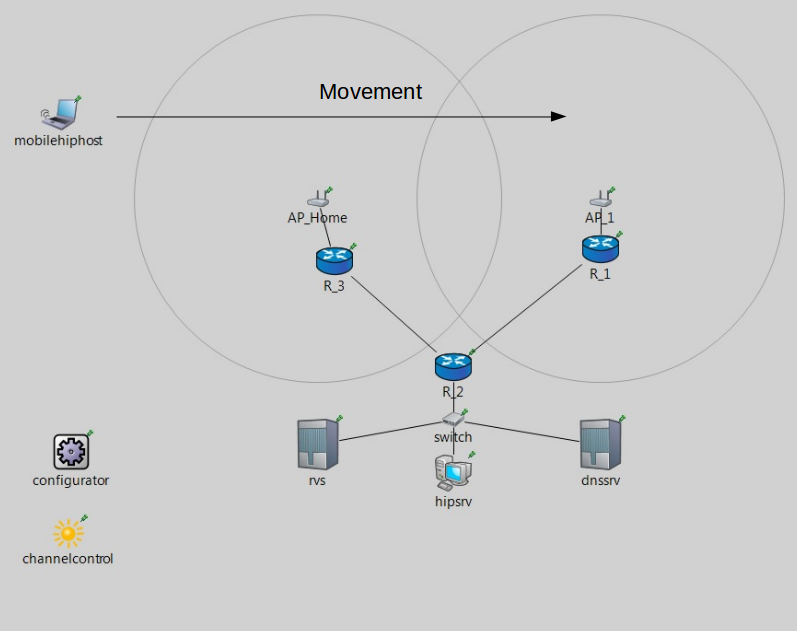
\includegraphics[scale=0.35]{c:/Users/Anu/Documents/images/hipmove.png}

\subsubsection{HIP}
The testbed for HIP is almost the same as MIPv6 as can be seen in the figure 2. Additionally it has two more nodes, namely ‘dnssrv’ and ‘rvssrv’ to enable the rendezvous mechanism, an extension of HIP to contact a frequently moving HIP node.  As per the rendezvous mechanism, both the HIP hosts hipsrv and mobilehiphost would register their HIT->IP address mappings with the Rendezvous Server (RVS) which in our case is ‘rvssrv’.  After this registration, the ‘rvssrv’ relays HIP packets arriving for these HITs to the node's registered IP addresses.  When a HIP node has registered with the ‘rvssrv’, it records the IP address of ‘rvssrv’ in its DNS record [5]. We statatically marked the ‘rvssrv’ in DNS for the HIP hosts in ‘dns.xml'.

\subsection{Mobility Management}
To evaluate the performance of the above mentioned protocols, we defined mobility scenarios in which we evaluated the handover latency experienced by mobile hosts when using HIP and MIPv6 respectively. Additionally, we also tested a multihoming scenario in which we evaluated the rehoming time experienced by a mobile host when using HIP. Note that multihoming is not supported in MIPv6, hence was tested it only using HIP.
The mobile node (in both cases) is programmed to move in a straight line from home network to foreign network at following three speeds:
\begin{enumerate}
\item Pedestrian – 5 km/h
\item In-Town – 40 km/h
\item Train speed – 200 km/h
\end{enumerate}

The mobile node in both scenarios perform the association and initial configuration once they reach in the range of their home network. Then they start sending the packets to the stationary node and continue moving away from the home network, towards foreign network. This movement eventually causes handover. The evaluation is based on following metrics: 

\subsubsection{Handover Latency for MIPv6}
For MIPv6, the handover latency is based on the binding update mechanism explained above. So we calculated the handover latency as elapsed time between the moment of association of the MN with the new access point and the instant MN receives the binding acknowledgement message from the Home Agent, measured in seconds for each of the mobility scenario.

\subsubsection{Handover Latency (Rehoming time) for HIP}
For HIP, the handover latency is evaluated based on the update mechanism explained above. So we calculated handover latency (and rehoming time) for HIP as the elapsed time between the moment of association of the ‘mobilehiphost’ with the new access point ‘AP\_1’ and the instant ‘hipsrv’ receives the third UPDATE message from the ‘mobilehiphost’, also measured in seconds for each of the scenario.

\section{Simulation Results and Analysis}
In this section, we present the results and analysis of the simulation experiments to implement the mobility scenarios explained above. Table 1 shows the mean values of handover latency and rehoming time observed in our experiments. Graph 1 shows a comparison in those values with time and speed. As can be seen from the results, HIP has a better overall average latency of 1.73 seconds as compared to 2.29 seconds for MIPv6. MIPv6 is slower because it involves more signalling [9]. Another observation here is that since the speed increases, the latency increases. Rehoming (as tested in HIP) performs way better (0.14 seconds) because of proactive IPv6 address configuration.  

\section{Conclusion}
Each protocol has its own advantages and disadvantages. Our simulation results clearly show that HIP has a better overall performance when it comes to handover latency and rehoming time. Additionally, HIP is inherently more secured than MIPv6. Despite low handover latency, HIP takes more time during association (key-exchange). Also, it involves addition of a new layer between network and transport layer and new network elements like RVS. Due to its signalling overhead MIPv6 performs slower in terms of handover latency, but does not need alteration of the network layer and it is integrated in the IPv6 specification.

%The bibliography, done here without a bib file
%This is the old BibTeX style for use with llncs.cls
\bibliographystyle{splncs}

\begin{thebibliography}{1}
%add each reference in here like this:
\bibitem[1]{}
Site: OpenSim Ltd. OMNET++ official site
Link: https://omnetpp.org/
Other info: (retrieved June 2016).


\bibitem[2]{}
Site: ICT-OPTIMIX, HIPSim++ framework for OMNET++ official site
Link: http://www.ict-optimix.eu/index.php/HIPSim
Other info: (retrieved June 2016).


\bibitem[3]{}
Site: INET Framework community site
Link: https://inet.omnetpp.org/ 
Other info: (retrieved June 2016).


\bibitem[4]{}
Authors: D. Johnson, C. Perkins, J. Arkko. 
Article: RFC 6275: Mobility Support in IPv6, IETF July 2011
Link: https://tools.ietf.org/html/rfc6275
Other info: (retrieved June 2016).


\bibitem[5]{}
Authors: J. Laganier, L. Eggert. 
Article: RFC 5204:  Host Identity Protocol (HIP) Rendezvous Extension, IETF April 2008
Link: http://www.ict-optimix.eu/index.php/HIPSim
Other info: (retrieved June 2016).


\bibitem[6]{}
Authors: P. Nikander, T. Henderson, Ed., C. Vogt, J. Arkko. 
Article: RFC  5206: End-Host Mobility and Multihoming with the Host Identity Protocol, IETF April 2008
Link: https://tools.ietf.org/html/rfc5206 
Other info: (retrieved June 2016).


\bibitem[7]{}
Authors: R. Moskowitz, P. Nikander, P. Jokela, Ed., T. Henderson. 
Article: RFC 5201: Host Identity Protocol, IETF April 2006
Link: https://www.ietf.org/rfc/rfc5201.txt 
Other info: (retrieved June 2016).

\bibitem[8]{}
Authors: C. Mugga, D. Sun. 
Article: Performance comparison of multihoming and mobility protocols in IPv6 heterogeneous network environment, Blekinge Institute of Technology, Sweden, October 2013.
Link: http://www.diva-portal.org/smash/get/diva2:830094/FULLTEXT01.pdf 
Other info: (retrieved June 2016).


\bibitem[9]{}
Authors: P. Reinbold, O. Bonaventure. 
Article: A Comparison of IP mobility protocols, Infonet group, University of Namur, Belgium.
Link: http://citeseerx.ist.psu.edu/viewdoc/downloaddoi=10.1.1.21.2328\&rep=rep1\&type=pdf  
Other info: (retrieved June 2016).

\bibitem[10] {}
Authors: H. A. Chan, O. E. Falowo, L. A. Magugala. 
Article: Handover approaches for seamless mobility management in next generation wireless networks
Book: Wireless Communications and Mobile Computing, vol. 12, no. 16, November 2012, pp. 1414-1428 

\end{thebibliography}
\end{document}